% Chapter 1

\chapter{Introduction} % Chapter title

\label{ch:introduction} % For referencing the chapter elsewhere, use \autoref{ch:introduction} 

%----------------------------------------------------------------------------------------



\minitoc

\section{Nuclear Energy in France}

In 2020, France had a total of 136.2~GW of installed electrical power plants with a total production over the year of 500.1~TWh, 67.1\% of which coming from nuclear reactor. Actually, nuclear energy plays a pivotal role in France's electrical mix since the 1950's and is promoted as a mean to reduce the global carbon dioxide emissions of the country's energy production. The french government currently plans to build a total of six new nuclear reactors before 2050.

%\begin{figure}[!h]
%\centering
%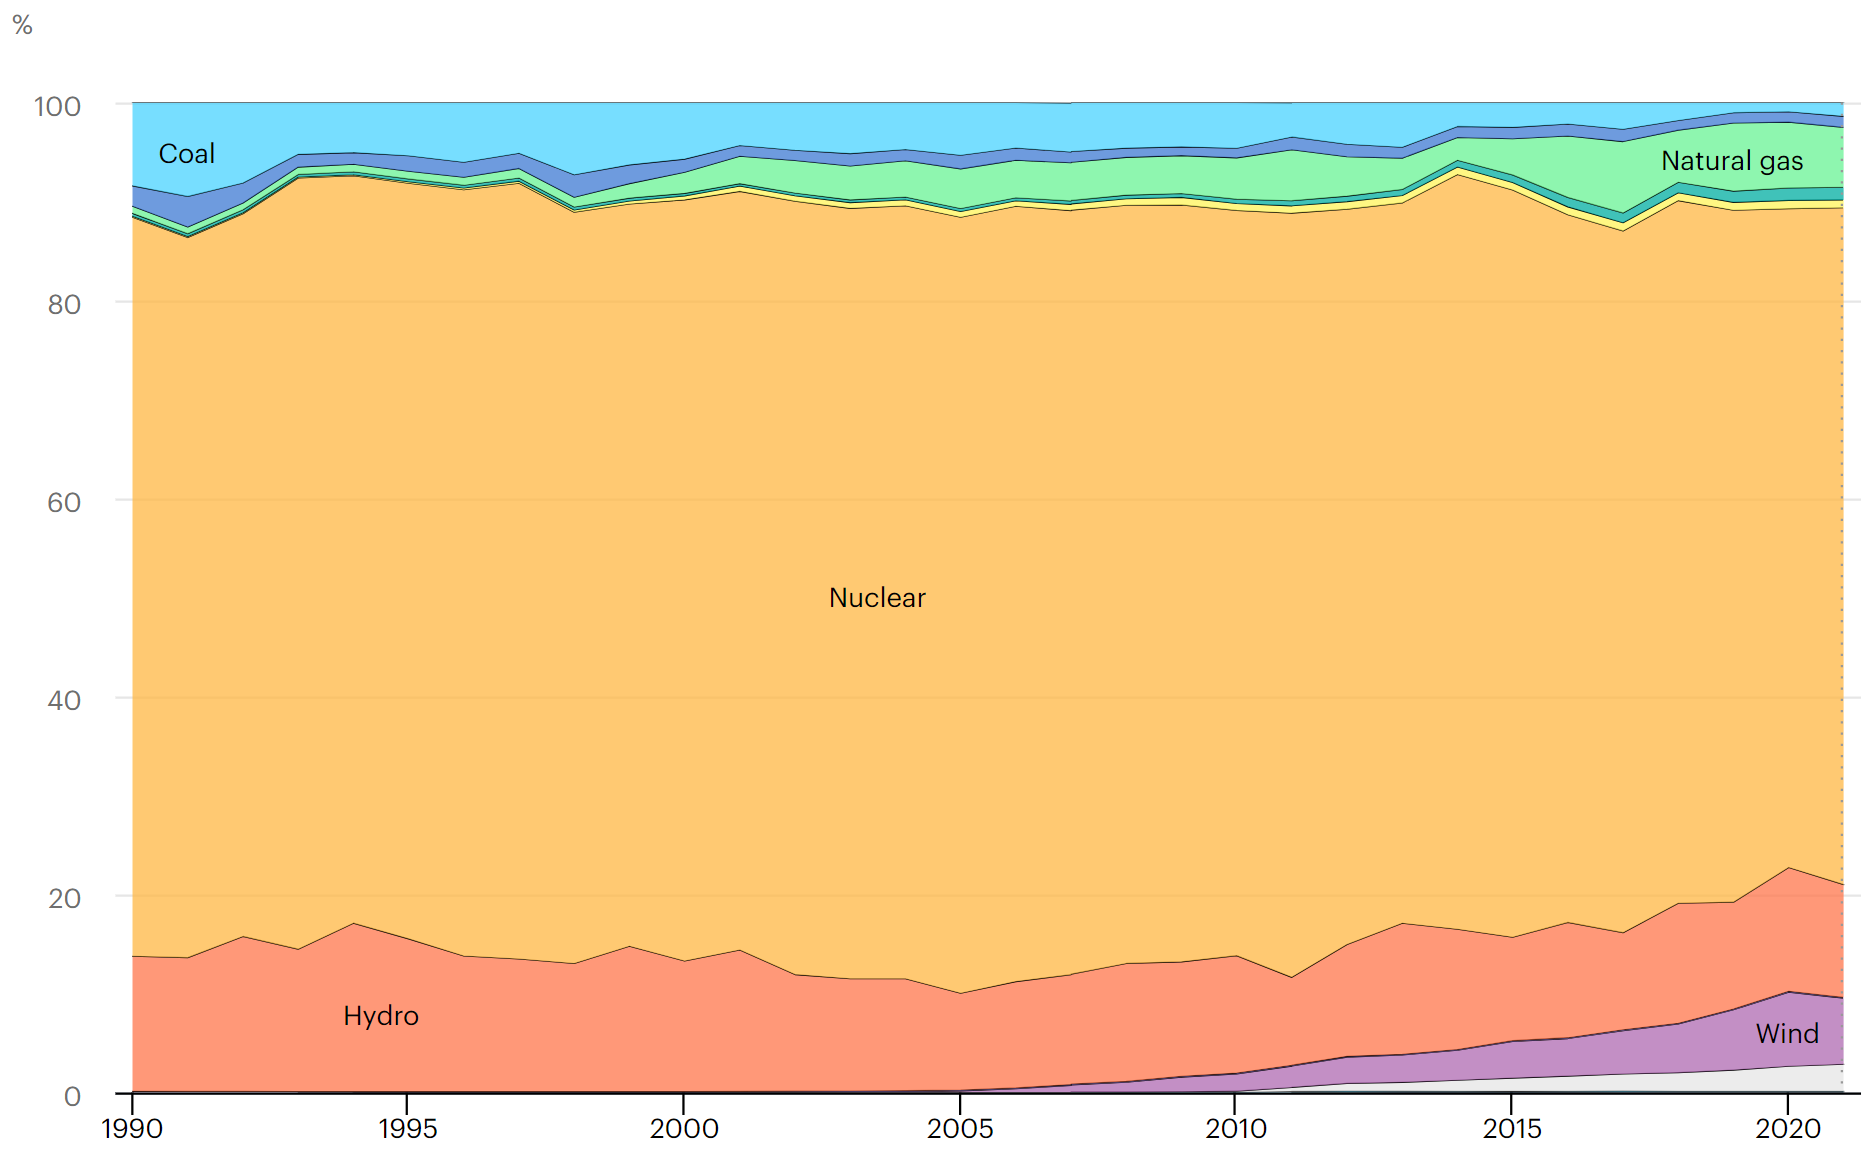
\includegraphics[width=0.8\linewidth]{img/intro/energy_france.png}
%\caption{Shared parts of electricity production in France between 1990 and 2021. \cite{iaea_france_nodate}. }
%\label{fig:france_energy_mix}
%\end{figure}

%\npar

%France accounts for a total of 56 nuclear power units in 2020, all being Pressurized Water Reactors (PWR). They are dispatched over 19 different geographic locations and split in three electrical power series:
%
%\begin{itemize}
%\item 900~MW series (32 units), launched between 1978 and 1988 (total installed power of 28.8~GW) ;
%\item 1300~MW series (20 units), launched between 1985 and 1994 (total installed power of 26.3~GW) ;
%\item N4 series (1450~MW, 4 units), launched between 2000 and 2002 (total installed power of 6~MW) being the most recent french PWR.
%\end{itemize}


%%%%FIGURE OF NUCLEAR POWER PLANTS MAP



\section{Physical and Technological Background}
%
%\subsection{Nuclear Energy}
%
%\subsubsection{Nuclear Fission}
%
%On earth only one isotope exists that is called "fissile" : uranium 235 (noted $^{235}U$). Under certain physical conditions, $^{235}U$ collision with a neutron results in its break-up in two lighter atoms while releasing a total of two to three neutrons and an energy of the order of 200~MeV ($\approx 3.2 \times 10^{-11}$\ J). This amount of energy results from the mass difference between the $^{235}U$ and the products of the fission (atoms and neutrons), which is transferred as kinetic energy to the latter (Figure \ref{fig:fission}).
%
%
%
%\begin{figure}[!h]
%\centering
%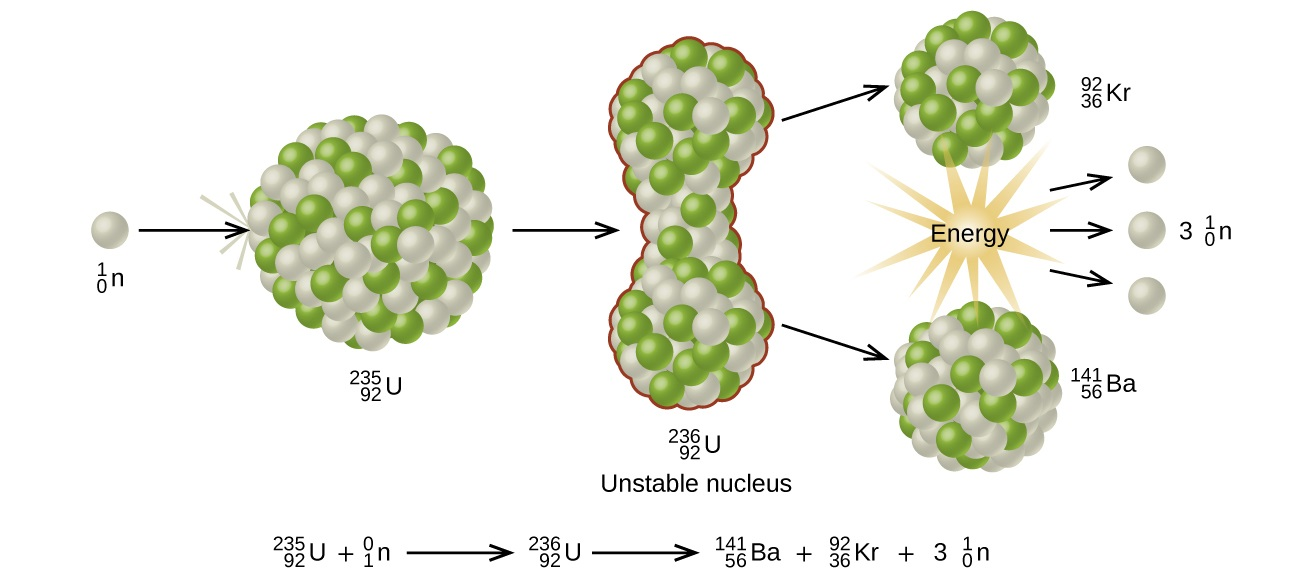
\includegraphics[width=0.7\linewidth]{img/intro/fission.jpg}
%\caption{Sketch of a nuclear fission process. \cite{chemistry_libretexts_217_2017}}
%\label{fig:fission}
%\end{figure}
%
%\npar
%
%$^{235}U$ used in PWR is an isotope of uranium and accounts for only 0.7\% of the common uranium found in nature, most of which being uranium 238 ($^{238}U$) that is not fissile. For nuclear power production, common uranium must be enriched in $^{235}U$ up to 3\% to 5\% \cite{croff_introduction_2008}.
%
%\subsubsection{Nuclear Chain Reaction and Energy Production}
%
%
%Fission presents particular interest for energy production due to its capacity to create a "nuclear chain reaction". Indeed, as multiple neutrons are expelled after the nuclear fission (Figure \ref{fig:fission}), each of them can potentially become a trigger for a new fission of a nearby $^{235}U$ atom. Since each fission releases more neutrons than required for its own triggering, this results in an exponentially increasing number of fissions called a nuclear chain reaction.
%
%\npar
%
%However, neutrons released by the fission can't directly trigger a new one. They are emitted with a kinetic energy of approximately 2~MeV at which the probability of impacting an other $^{235}U$ is too low to start the nuclear chain reaction. Therefore, a so-called "moderator" is needed to slow down the neutrons through collisions with other atoms. Then the fission reactions lead the nuclear fuel to heat up rapidly and needs to be cooled to evacuate the produced energy. Using a fluid, it must both act as a coolant and allow the nuclear chain reaction to continue (moderator role). In french PWR, this is achieved using water as cooling fluid which also moderates the neutrons going through it.
%
%\begin{remark*}{}
%Other nuclear reactor technologies exist with different fluids such as gas-cooled reactors using graphite as moderator material and carbon dioxide as coolant.
%\end{remark*}
%
%\npar
%
%Following the heat exchange between the nuclear fuel and the water, the thermal energy stored in it can be used in a thermodynamic cycle (\eg Hirne cycle) to produce electrical power.



\subsection{Pressurized Water Reactor Operation}

Pressurized Water Reactors are the only type of nuclear power plants operated in France for electricity production. A simplified sketch of a PWR is presented on Figure \ref{fig:pwr_sketch}.

\begin{figure}[!h]
\centering
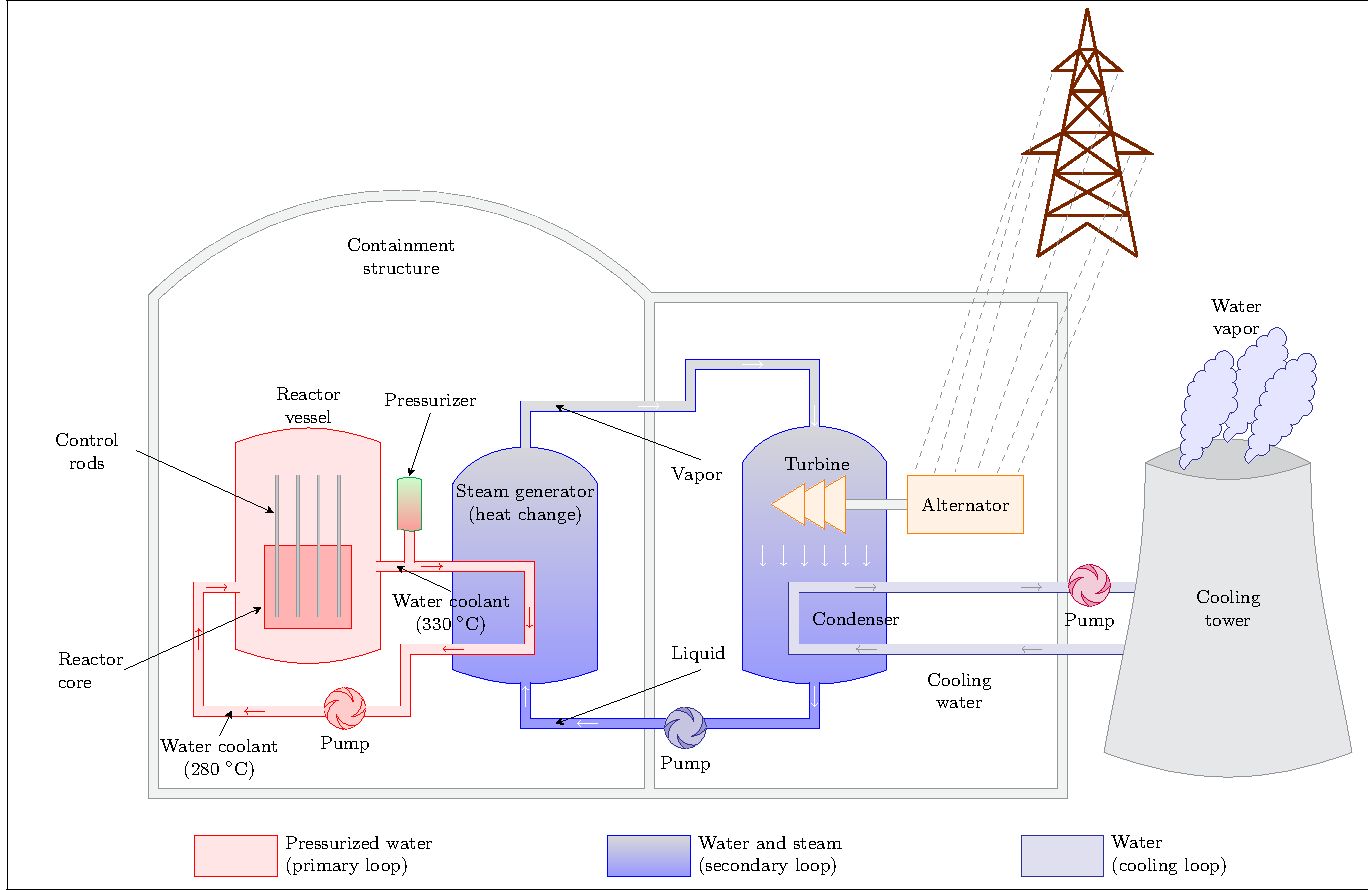
\includegraphics[width=1.0\linewidth]{img/intro/pwr_tikz.pdf}
\caption{Sketch of a Pressurized Water Reactor \cite{faccanoni_etude_2008}}
\label{fig:pwr_sketch}
\end{figure}

\npar

\subsubsection{Primary Loop}

The primary loop aims to collect the thermal energy expelled by the fission reactions within the nuclear fuel rods. The water flowing through the core gathers this energy and transfers it towards the vapor generator, while ensuring a moderating effect to maintain the nuclear chain reaction in the fuel. The primary loop is fully closed and operates at a pressure around 155\ bar, a temperature of $300\degC$ and mass flow rates between $3000$ and $5000\ \debm$ (approximately 20 tons per second) at the core inlet.  

\npar

The reactor vessel is fed with water by numerous pumps, each of them being connected to its own cooling circuit and steam generator. One of those coolant circuit is connected to the pressurizer to set the pressure of the whole primary loop. In France, 900~MW reactors comprise three primary pumps while 1300~MW and 1450~MW reactors have four of them.

\npar

The main components of the primary loop are:

\begin{itemize}
\item \textbf{The reactor vessel} containing the core where fission reactions take place within the nuclear fuel rods, gathered in so-called "fuel assemblies". The pressurized water flow between the rods to remove the heat released at their surface and moderates the neutrons to maintain the chain reaction.

\item \textbf{The primary pumps} which role is to ensure the water flow throughout the loop. Each pump requires an electrical power supply of approximately 7~MW.

\item \textbf{The pressurizer}, imposing the pressure and keeps the water in a liquid state. It is actually a vessel with a liquid-vapor mixture in which pressure can be increased through vaporization of the liquid water (using heating resistors) or diminished by vapor condensation (using water aspersion system).

\item \textbf{Steam generator tubes} being the interface between the primary and secondary loop through which the thermal energy gathered in the core is transferred from the primary water to vaporize the secondary water.
\end{itemize}


\subsubsection{Secondary Loop}

The secondary loop is designed to receive the thermal energy from the primary loop to vaporize its own water. The generated vapor is used to produce electricity by conversion of its mechanical energy through the rotation of power-generating turbines connected to alternators. At the outlet of the turbines, the vapor has logically been expanded and is then condensed before being sent back into the secondary loop and the steam generators. Therefore, the secondary loop is a closed water-steam circuit. The operating conditions in the steam generator are usually a pressure of 60 bar, with water heated from $220\degC$ to $275\degC$ and evaporated.

%\npar
%
%Main components of the secondary loop are:
%
%\begin{itemize}
%\item \textbf{Steam generators} in which water flows around tubes containing the primary water and gets evaporated.
%
%\item \textbf{High and low pressure turbines} which role is to transfer the mechanical energy contained in the steam towards the alternators. First, the high pressure part expands the steam from 60 bar to 10 bar before the low pressure part decreasing the pressure down to 0.05 bar. The use of two-stage expanders increases the global thermodynamic efficiency of the cycle.
%
%\item \textbf{The condenser} connecting the secondary loop and third (cooling) loop by operating the heat exchange dedicated to vapor condensation at a pressure of 0.05 bar. The condensation relies on the external heat sink of the cooling loop.
%\end{itemize}
%
%
%For a reactor producing an electrical power of 900~MW, the remaining thermal power to evacuate through the condenser after the low-pressure turbine stage lies around 1800~MW.


\subsubsection{Cooling Loop}


The cooling loop's goal is to cool down and condense the steam coming out of the turbines. Depending on the geographical situation of the nuclear power plant, the associated heat sink may either be natural (lake, sea, etc.) or built (cooling tower). It is a completely open circuit.

%:
%
%
%\begin{itemize}
%\item \textbf{A cooling tower} cools down and condenses vapor by direct contact with outdoor air. Most of the condensed water falls down the tower and is further re-injected in the loop, while the remaining part escapes into the atmosphere as a steam cloud. This loss of water is compensated by pumping from local natural source (usually a river).
%
%\item \textbf{A natural heat sink} (\eg a sea) is self-sufficient to act as an "infinite" cold source. Water is then directly pumped from it and injected in the condenser to extract the heat from the secondary circuit before being sent back. The level of heating of the natural source is controlled following environmental policies. 
%
%\end{itemize}
%
%
%The cooling loop is thus a completely open circuit.


\subsection{Structure and Geometry of PWR Core}


\subsubsection{Reactor Pressure Vessel}

The whole reactor core is contained in a stainless steel vessel (Figure \ref{fig:vessel_pic}) called "Reactor Pressure Vessel" (RPV). Together with the primary loop, they represent the second "containment barrier" (name given to the parts of the reactor avoiding the escape of radioactive species) of the core. Therefore, the RPV is a pivotal safety element of the reactor which mechanical strength and performances must be ensured in any conditions that may occur during operations.

\begin{note*}{}
A RPV can not be replaced, thus scaling the whole reactor's lifetime. The longer the vessel is durable, the longer the nuclear unit will operate.
\end{note*}




\begin{figure}[!h]
\centering
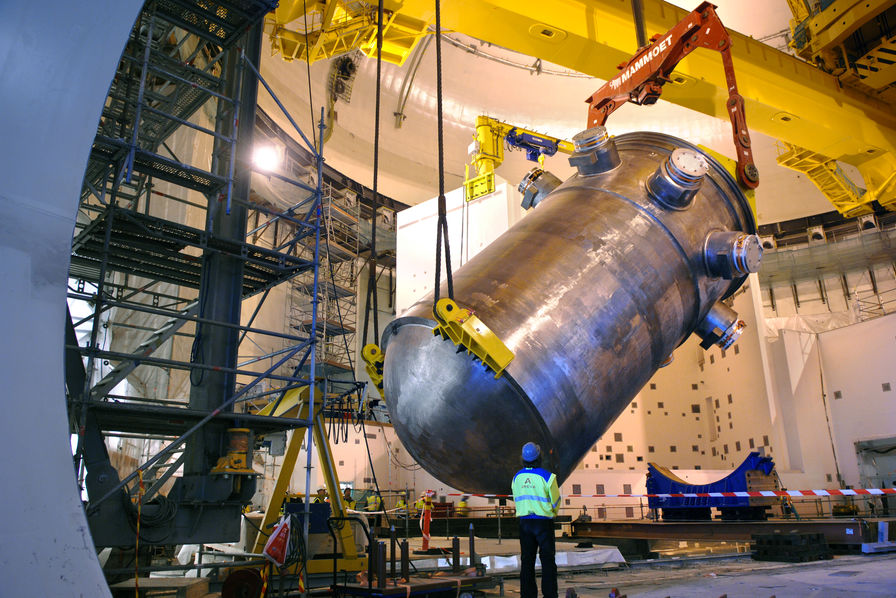
\includegraphics[width=0.6\linewidth]{img/intro/vessel_pic.jpg}
\caption{Picture of the Reactor Pressure Vessel of the Finnish European Pressurized Reactor \cite{nouvelle_cuve_2010}, \textcopyright Areva}
\label{fig:vessel_pic}
\end{figure}

\npar


\subsubsection{Fuel Assembly and Core Structure}

A fuel assembly is composed of $17 \times 17$ rods and guide thimbles among which 264 are nuclear fuel rods. 24 of them are guide thimbles in which absorbing rods (used to shut down the chain reaction by neutron absorption in incidental or accidental situations) can be inserted, one of them being dedicated to instrumentation. The top nozzle of the assembly ensures its stability using a hold-down spring. The whole structure is 4\ m high and is also maintained by 8 grids placed every 50\ cm (Figure \ref{fig:fuel_assembly}) for french PWR reactors. 



\begin{figure}[!h]
\centering
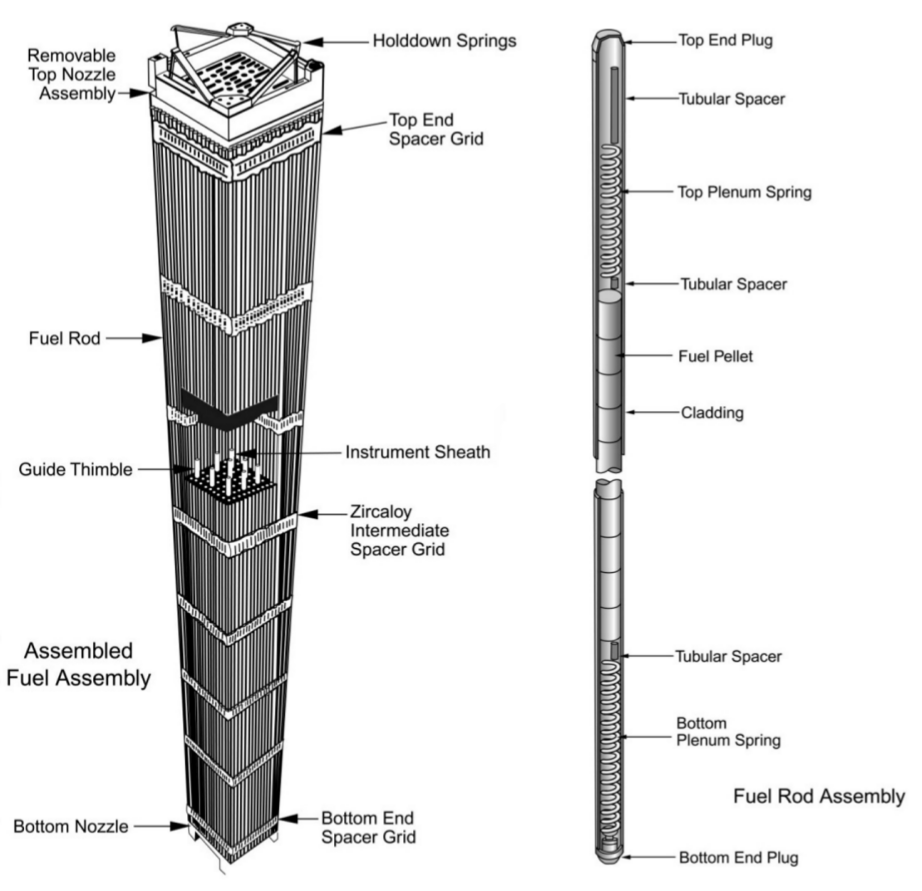
\includegraphics[width=0.7\linewidth]{img/intro/fuel_assembly.png}
\caption{Sketch of a full nuclear fuel assembly and rod. \cite{croff_introduction_2008}}
\label{fig:fuel_assembly}
\end{figure}

\npar

In a reactor core, the number of fuel assemblies can vary depending on its final electrical power production: 157 assemblies for 900\ MW units, 193 for 1300~MW units and 205 for 1450~MW units.

\subsubsection{Fuel Rod}

Fuel rods are the elementary component of the reactor's core since they contain the nuclear fuel pellets made of enriched uranium. A pellet measures 13.5\ mm height for an 8\ mm diameter, weighing approximately 8.3\ g. They are placed in a neutron-transparent tubular cladding made of Zircaloy (an alloy made of 98\% of zirconium and tin), allowing neutrons to move through the core to trigger fission reactions in nearby rods. This cladding is the first containment barrier and contains a total of 272 pellets (Figure \ref{fig:fuel_assembly}).

\npar

The bundle organization of the rods allows water to flow between them and to moderate neutrons coming out of recent fission. Moreover, this geometry ensures a large heat exchange surface to enhance the fuel cooling. A single fuel rod usually measures 4\ m height for a 9.5\ mm diameter and weighs 2\ kg (Figure \ref{fig:fuel_rod}).


\begin{figure}[!h]
\centering
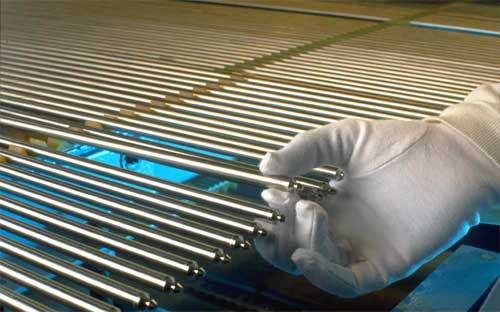
\includegraphics[width=0.6\linewidth]{img/intro/fuel_rod.jpg}
\caption{Picture of a fuel rod during a control test. \cite{kamin_cycle_2019}}
\label{fig:fuel_rod}
\end{figure}

\npar

\begin{note*}{}
In normal PWR conditions, the heat flux at the rods lies roughly between $500~$kW/m\up{2} and 1.5~MW/m\up{2} \cite{pujet_memento_2016}. In accidental conditions, it can rise up to several MW/m\up{2} \cite{manon_contribution_2000}.
\end{note*}
 
\subsubsection{Grids}

Within the fuel assembly, the rods are held by 8 grids (Figure \ref{fig:fuel_grid}) placed with an even spacing of 50\ cm. 

\begin{figure}[!h]
\centering
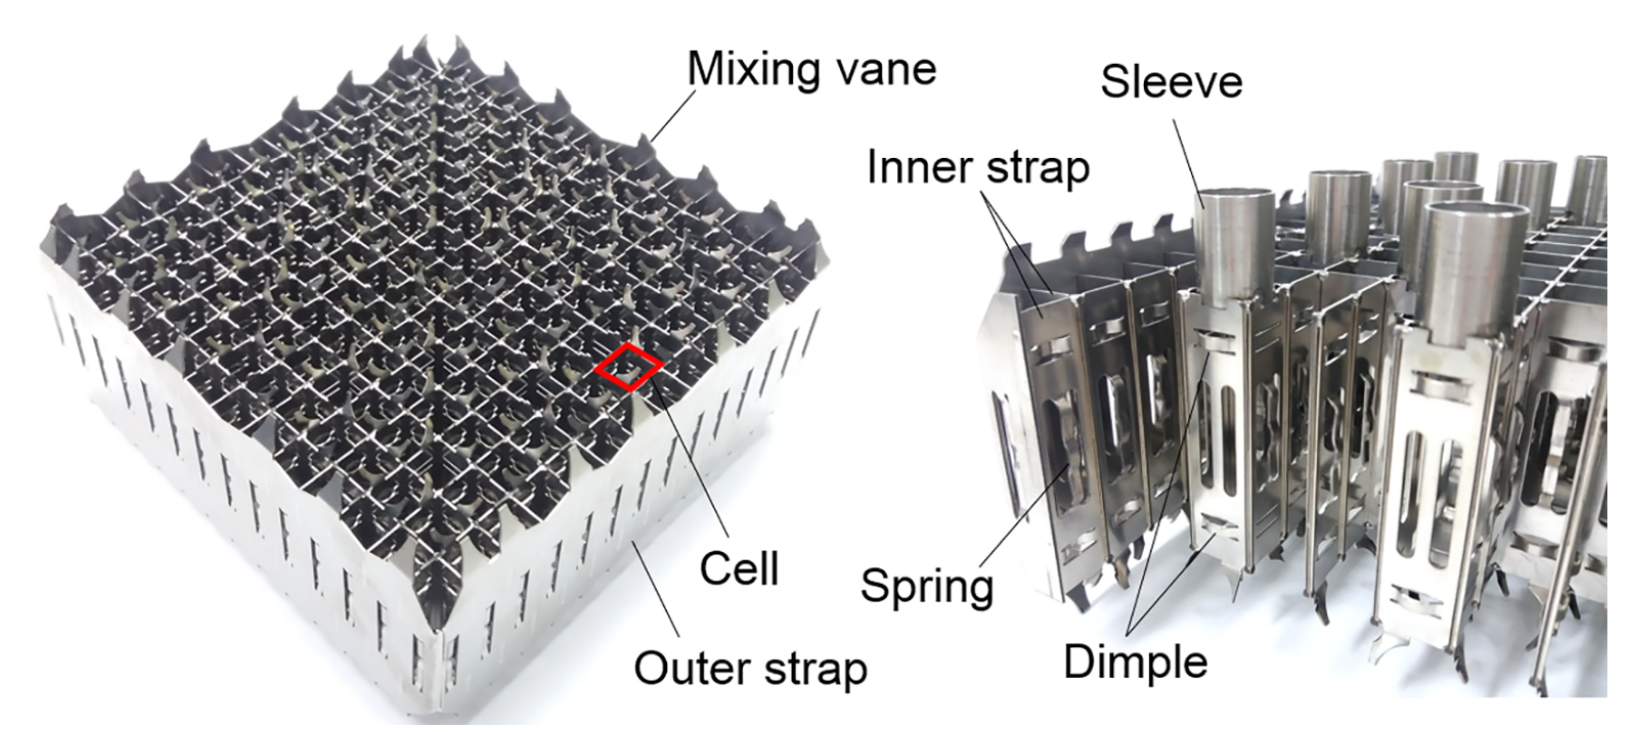
\includegraphics[width=0.8\linewidth]{img/intro/pic_grid.png}
\caption{Picture of a fuel assembly grid. \cite{yoo_finite_2019}}
\label{fig:fuel_grid}
\end{figure}

\npar


They help the whole structure to withstand the huge hydrodynamic effort exerted by the water flowing over the rods
at high flow rates. Two types of grids are used in fuel assemblies:

\begin{itemize}
\item Spacer grids which role is solely to ensure the mechanical stability of the assembly and avoid rods deformation when they heat up.
\item Mixing grids equipped with mixing vanes (Figure \ref{fig:fuel_grid}) that adds a rotational motion to the axially flowing fluid enhancing the turbulence and mixing to homogenize its temperature.
\end{itemize}

Figure \ref{fig:fuel_grid_I8C} shows an enlarge model of a grid for a $5 \times 5$ rod bundle. The 25 cells holding the rods are clearly visible along with the different components being the mixing vanes, the dimples and the springs. The latter two holding the rods straight when they are inserted through the grid.


\begin{figure}[!h]
\centering
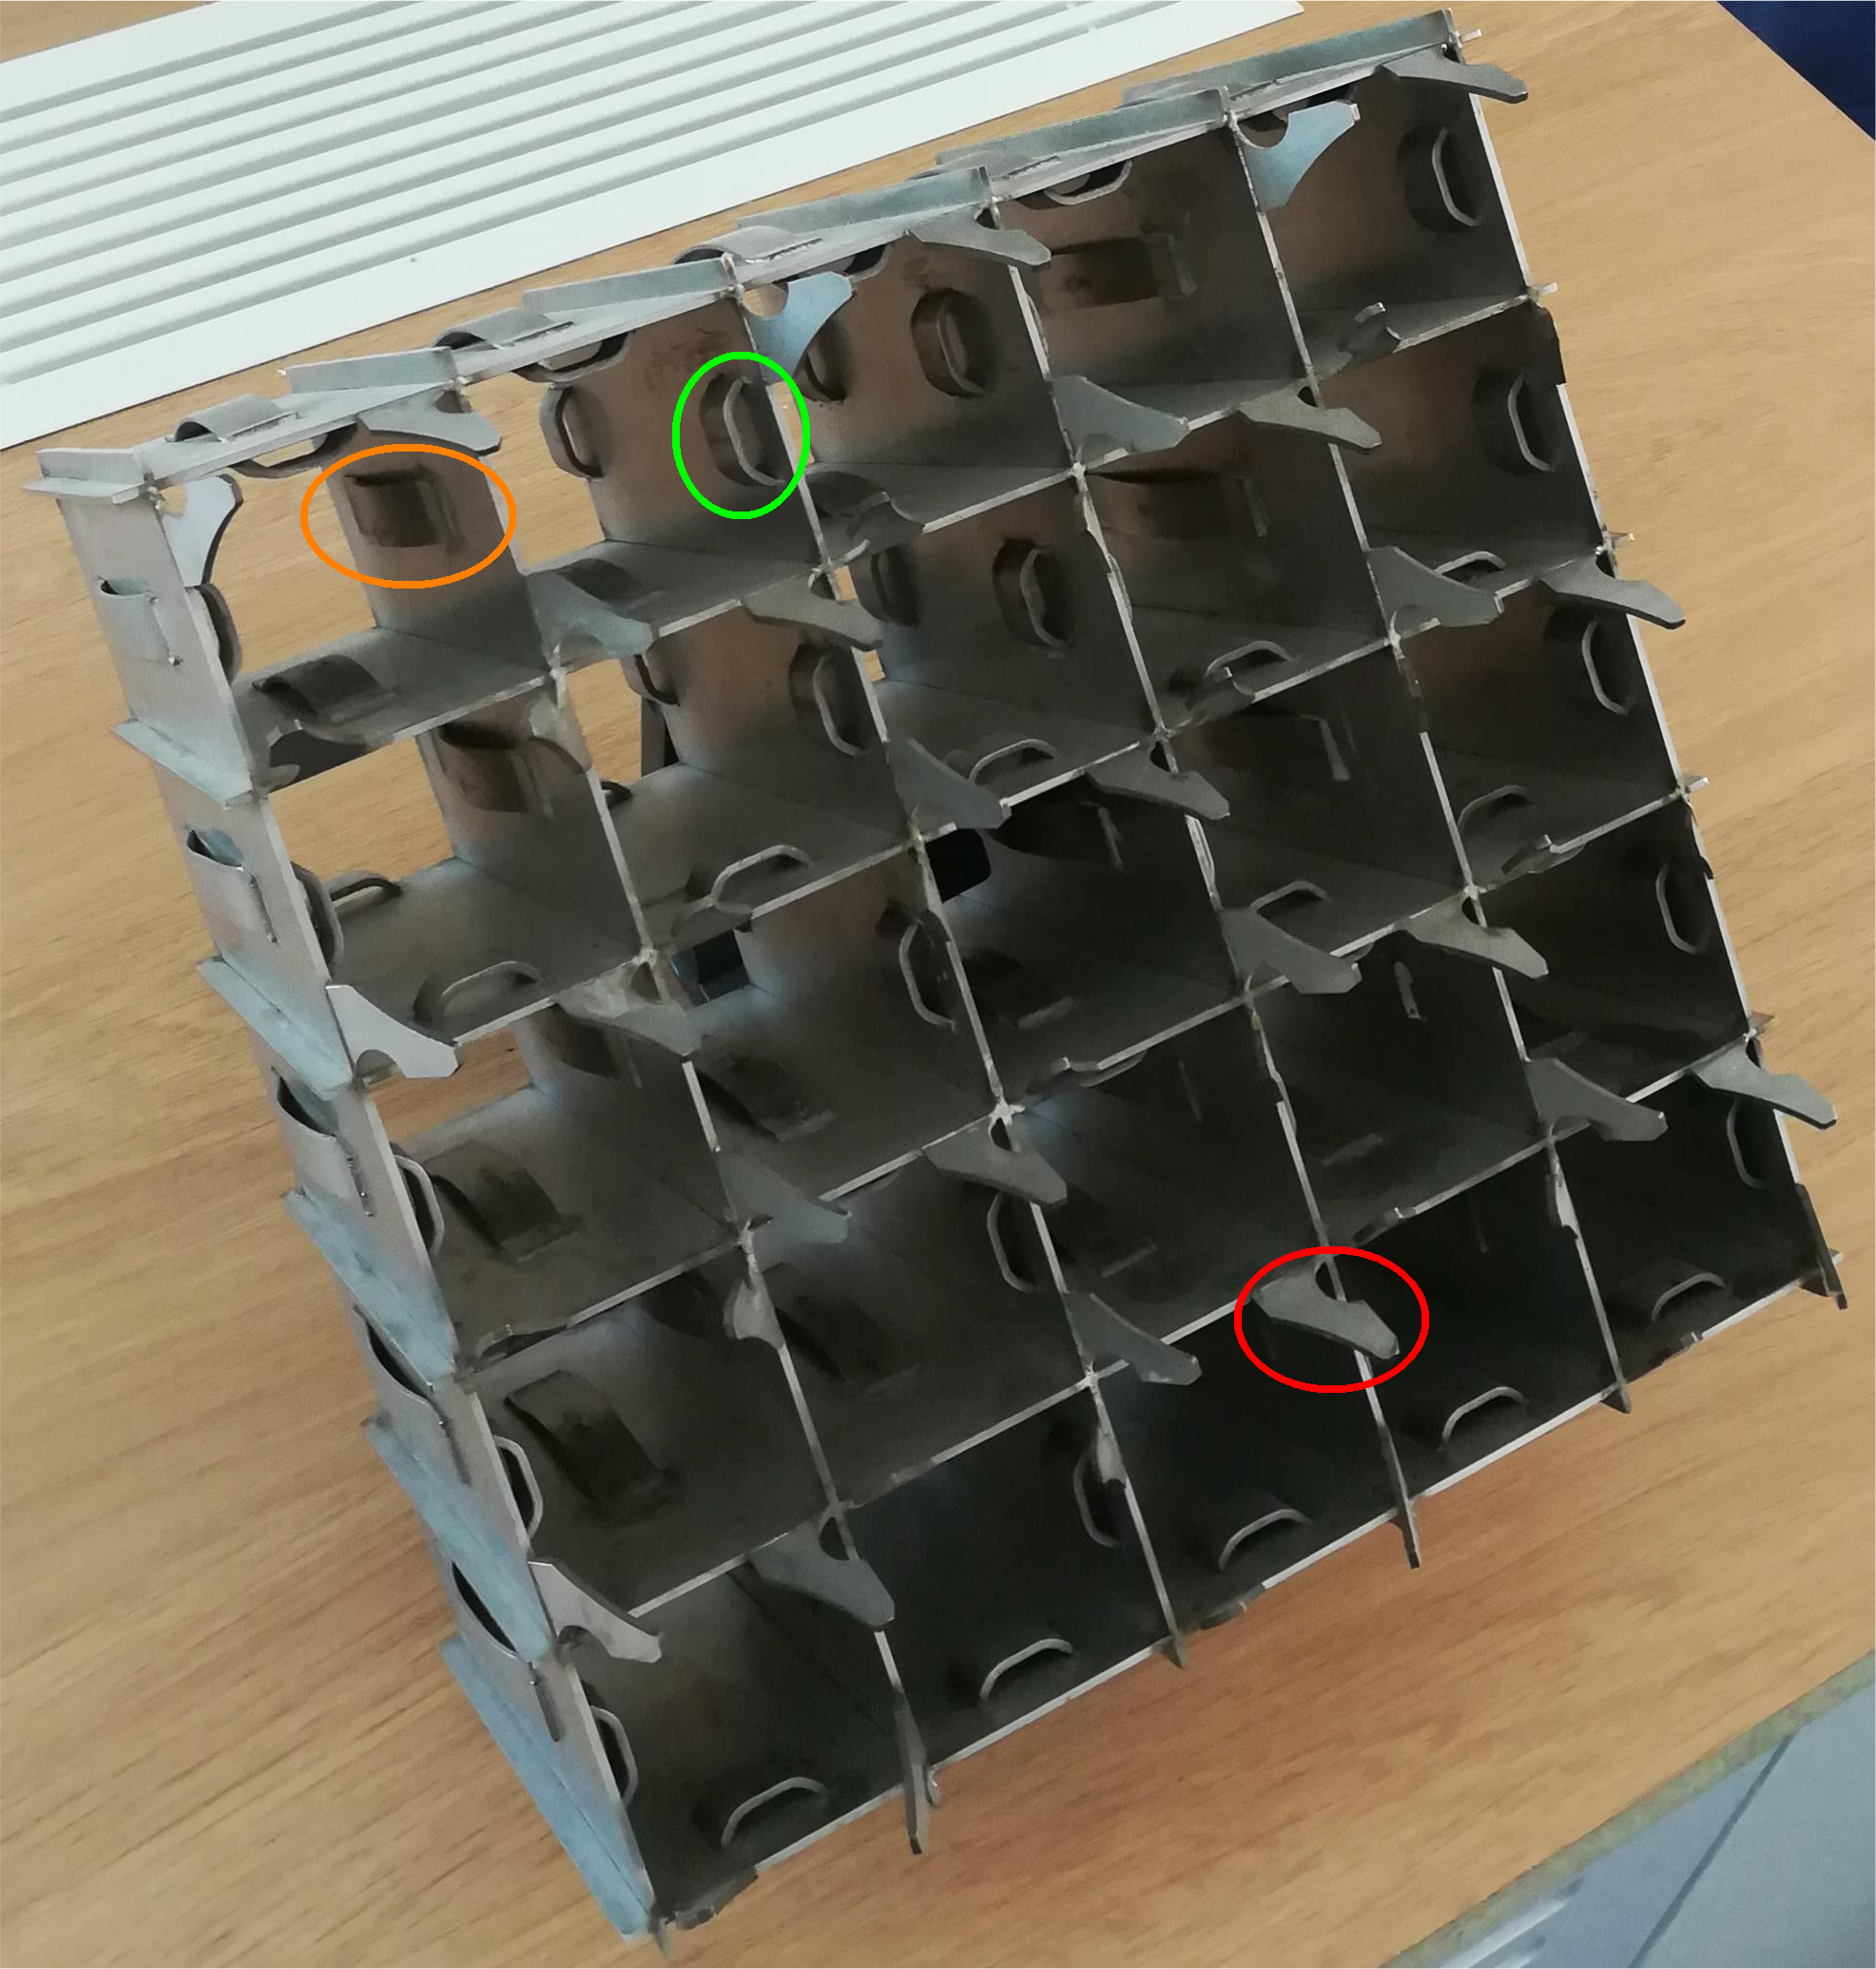
\includegraphics[width=0.3\linewidth]{img/intro/MaquetteGrille.png}
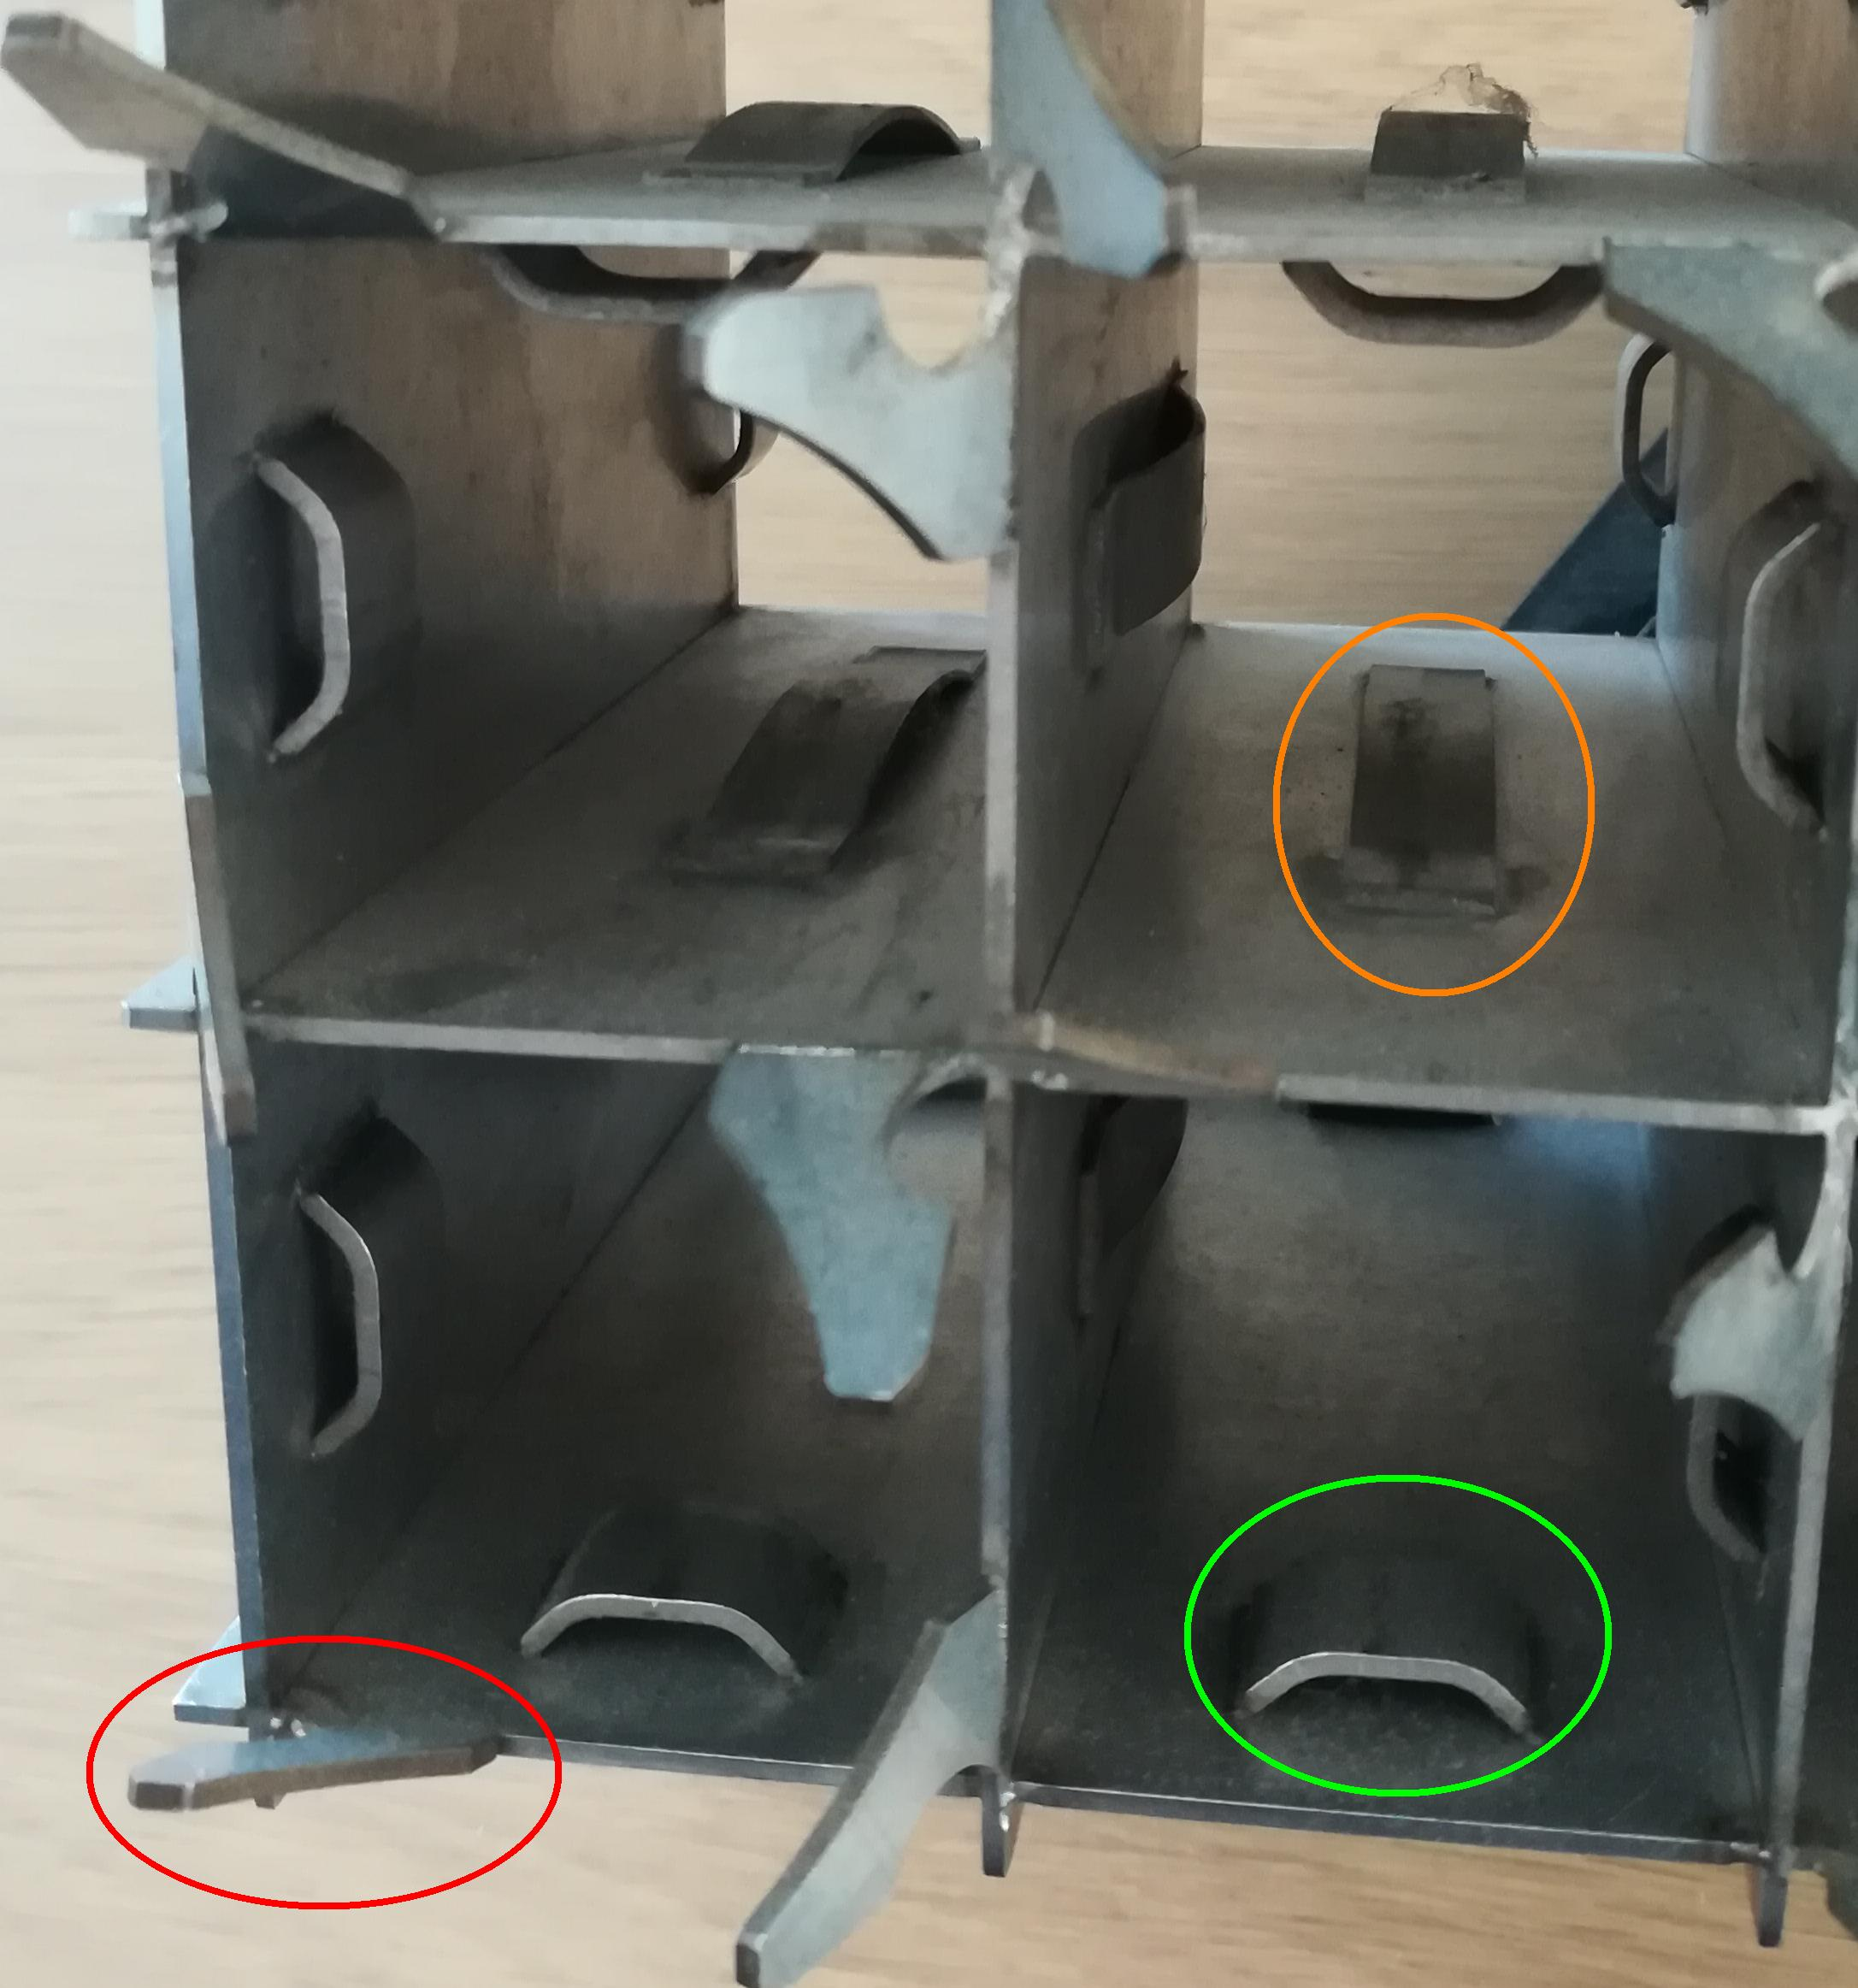
\includegraphics[width=0.3\linewidth]{img/intro/CanauxGrille.jpg}
\caption{Model of a $5 \times 5$ grid (scale 5:1) from EDF Lab Chatou. Mixing vanes circled in red, dimples in green and springs in orange.}
\label{fig:fuel_grid_I8C}
\end{figure}

\npar

\section{Safety and Thermal Design of PWR}

Regarding radioactivity, the safety of a PWR is ensured by three containment barriers:

\begin{itemize}
\item The fuel rod cladding (Figure \ref{fig:fuel_assembly}) ;
\item The Reactor Pressure Vessel and primary loop (Figure \ref{fig:vessel_pic}) ;
\item The containment building (Figure \ref{fig:pwr_sketch}).
\end{itemize}


Therefore, thermal-hydraulic design of a PWR has to account for any situation that can potentially pose a threat to those containment barriers. In particular, the water used as coolant in the core has to be able to remove the heat from the fuel rods in conditions being nominal, transient and also incidental. The different elements of the primary loop involved in the cooling process both have to be able to withstand the possible violent dynamic changes during the operation of the reactor and avoid to damage other parts of the circuit, especially those related to a containment barrier (fuel rods, RPV, etc.).

%
%\npar
%
%Two different types of accident are usually considered when designing the reactor core:
%
%\begin{itemize}
%\item The Loss Of Coolant Accident (LOCA) due to a rupture of a pipe connected to the primary loop leading to a pressure decrease that can vaporize the primary water. This accident is quite slow (from a few minutes to hours) and triggers an instant drop of the control rods to stop the nuclear chain reaction. A residual power (representing roughly 6\% of the nominal power) still has to be removed from the core.
%
%\item The Reactivity-Initiated Accident (RIA) corresponding to an abrupt rise of the nuclear activity of the fuel rods. This can happen under a failure of the hold-down springs (Figure \ref{fig:fuel_assembly}) leading to an ejection of the control rods. In this situation, the extremely fast transient regime (from a few milliseconds to seconds) lead to a quasi-instantaneous increase of the heat flux in the rods, resulting in their thermal expansion and presenting a high risk of fuel cladding damage. 
%\end{itemize}
%

In incidental conditions, the water around the fuel rods can be exposed to a huge increase of the thermal power it receives per unit of volume and being heated up above its saturation temperature, starting its vaporization. This can then lead to multiphase boiling flow regimes in the core, with a risk of reaching the critical situation called the \textbf{\underline{boiling crisis}} (BC).

\npar

The Boiling Crisis (described in the next Section) is among the most important thermal-hydraulic phenomenon that has to be accounted for in the design of nuclear reactors since it can severely damage the nuclear fuel rods cladding and thus requires dedicated studies and modeling. %For nuclear fuel assemblies, the physical situation consequently relates to vertical subcooled boiling flows.


\section{Thermal-Hydraulics of Boiling Two-Phase Flows}

In nuclear reactors, the water enters in the fuel assemblies from bottom and flows upwards while being heated along the 4~m height of the rods. It is initially highly subcooled \ie at a temperature $T_{L,in}$ much below the saturation temperature (usually a difference of $\Delta T_{L} = T_{sat}-T_{L,in} \approx 50 \degC$, $T_{sat} \approx 345\degC$ at 155\ bar) and exits the fuel assembly at $\Delta T_{L} = 15\degC$. Therefore, the physics at stake relates to \textbf{vertical subcooled boiling flows}.


\subsection{Vertical Subcooled Boiling Flow Regimes}

When the liquid heats up while flowing upwards, different heat exchange regimes can occur along with various multiphase flow regimes during phase-change. They are usually defined depending on the liquid thermodynamic quality $x_{eq} = \dfrac{h_{V,sat}-h_{M}}{h_{V,sat}-h_{L,sat}}$ ($x_{eq}<0$ if the the flow is subcooled, $0 \leq x_{eq} \leq 1$ if the mixture is at saturation) and the time-space distribution of the liquid and vapor phases. In the case of a simple tube, Figure \ref{fig:boiling_collier} presents a sketch of the different flow and heat transfer regimes occurring for vertical flow boiling in a tube with a negative inlet liquid quality. A low but constant heat flux is applied over the tube, long enough to end-up with pure vapor flow ($x_{eq} \geq 1$).


\begin{figure}[!h]
\centering
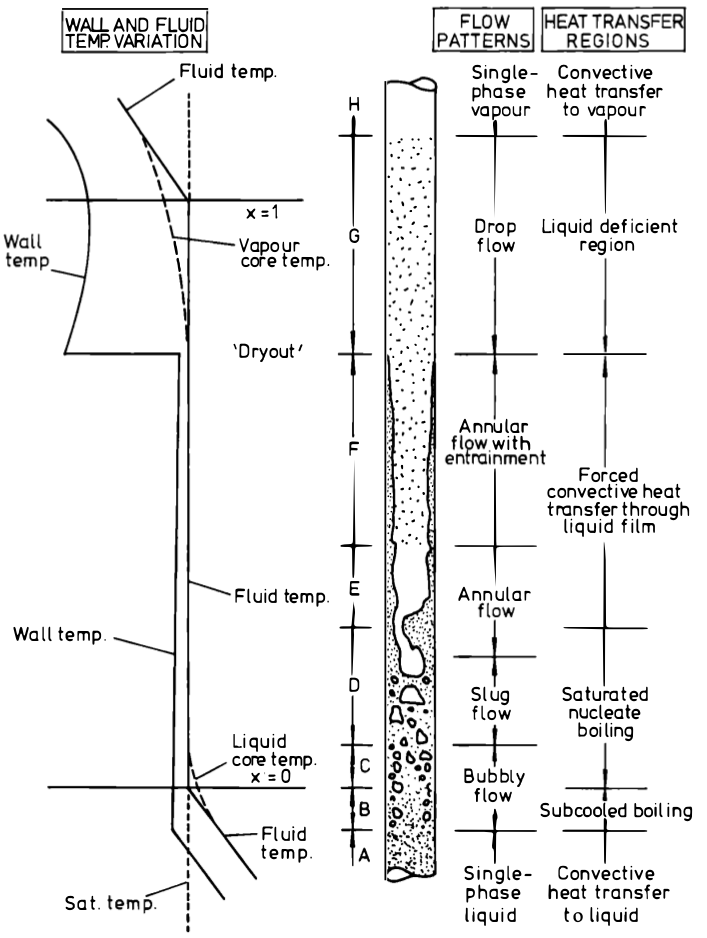
\includegraphics[width=0.6\linewidth]{img/intro/boiling_collier.png}
\caption{Sketch of the different vertical flow boiling regimes in a vertical tube at low heat flux from Collier \& Thome (1994, \cite{collier_convective_1994}). Here, $x$ denotes the local thermodynamic quality noted $x_{eq}$ in the text. }
\label{fig:boiling_collier}
\end{figure}


\npar


First, the liquid enters in a subcooled state \ie below saturation temperature, leading to a pure \textit{liquid convective heat transfer} (zone A).

\npar

Then, the wall heats up above the saturation temperature to reach the \textbf{Onset of Nucleate Boiling} (ONB), allowing vapor bubbles to nucleate at the wall on so-called "nucleation sites" (which density increases with the heat flux or wall temperature). This happens first in regions where the average temperature of the fluid is still below the saturation temperature, thus called \textit{subcooled boiling} (zone B). As we move upwards the tube, the boiling intensifies and bubbles start to leave the wall, corresponding to the \textbf{Onset of Significant Void} (OSV). They migrate into the bulk flow where they condense due to the locally subcooled liquid. In this region, the multiphase vapor-liquid flow is qualified as \textit{bubbly flow} and the vapor phase can be considered as dispersed into the main continuous liquid phase.

\npar

When the average liquid temperature reaches saturation, $x_{eq} = 0 $ and we enter the \textit{saturated boiling} regime. The vapor phase is first still composed of small dispersed bubbles in the bulk flow (zone C). Since liquid is at saturation temperature, vapor bubbles do not condense anymore and start to coalesce with each other, forming larger inclusions leading to a \textit{slug flow} (zone D).

\npar

Further downstream, the volume occupied by vapor at a given height starts to overcome that of the liquid phase \ie we reach high local "void fractions" (ratio of the vapor volume over the total volume). This leads to a significant change in the flow regime where the core flow is composed of vapor while liquid is pushed towards the wall, called \textit{annular flow}.  The liquid film trapped between the vapor and the wall increases the effective thermal conductivity and limits the possibilities of wall nucleation (zones E \& F).


%, corresponding to a phase inversion that defines the beginning of the \textit{annular flow} regime.

%During the transition from slug to annular flow, the heat transfer regime changes from saturated boiling (where bubbles merge in the bulk with the dominant vapor phase) to \textit{forced convective heat transfer through liquid film} (zone E). The forced convection in the film transports the heat from the wall to the liquid-vapor interface at which evaporation occurs, increasingly shrinking the liquid layer. The turbulence also tears off liquid droplets that are ejected in the bulk vapor flow, corresponding to the \textit{annular flow with entrainment} region.

\npar

Finally, when the liquid film has totally evaporated, the wall is in direct contact with the vapor phase (zones G \& H). This phenomenon is called \textbf{dryout} and is associated to a steep increase of the wall temperature due to the decrease of the heat transfer coefficient induced by the low vapor thermal conductivity.% Before reaching a pure vapor single-phase flow (zone H), liquid droplets can still exist in the bulk event passed the dryout, where we thus have a \textit{droplet flow} (zone G).


\subsection{Boiling Crisis and Critical Heat Flux in PWR}


The rapid rise of the wall temperature when dryout occurs actually corresponds to the so-called \textbf{boiling crisis}. The example of Figure \ref{fig:boiling_collier} shows the occurrence of a boiling crisis triggered by the evaporation of a thin liquid film separating the bulk vapor and the wall, called \textbf{Liquid Sublayer Dryout} (LSD), happening at low heat fluxes and high outlet quality ($x_{eq} >0.2$ usually). 

\npar

However in PWR, the very low inlet flow quality ($T_{L,in}\approx T_{sat}-50\degC$) combined with the high heat flux at the rods can trigger a boiling crisis of different nature. If the wall boiling becomes too intense, it may result in the formation of a vapor blanket at the wall insulating it from the liquid water cooling (Figures \ref{fig:dnb_bloch} and \ref{fig:dnb_liu}), thus abruptly increasing its temperature and posing a high risk of material damage. This type of boiling crisis is called the \textbf{Departure from Nucleate Boiling} (DNB). The heat flux at which the boiling crisis occurs is named \textbf{Critical Heat Flux} (CHF).


\begin{figure}[!h]
\centering
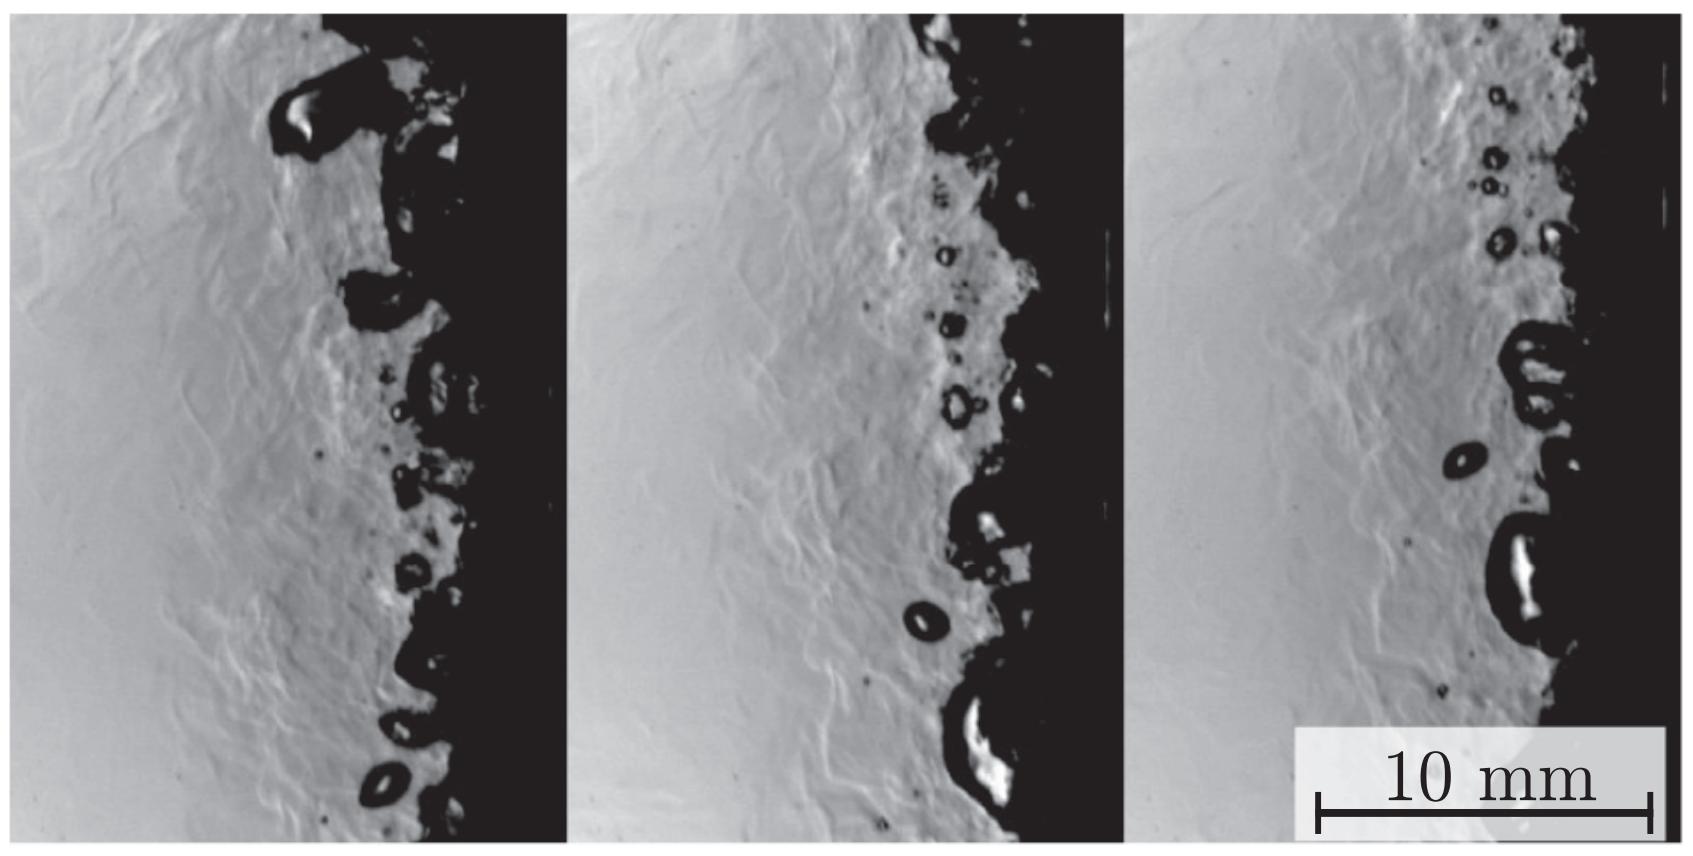
\includegraphics[width=0.5\linewidth]{img/intro/dnb_bloch.png}
\caption{Experimental shadowgrams from Bloch \etal \cite{bloch_phenomenological_2013} of the flow boiling at CHF for a 27\ K subcooled liquid flowing upwards at 0.6\ m/s and atmospheric pressure.}
\label{fig:dnb_bloch}
\end{figure}

\begin{figure}[!h]
\centering
\subfloat[$\phi_{w}\approx 0.96 \phi_{w,CHF}$]{
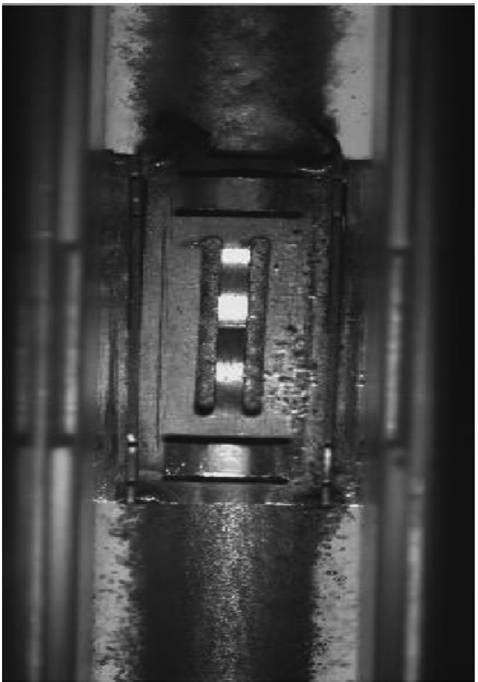
\includegraphics[width=0.25\linewidth]{img/intro/liu_96CHF.png}
}
\subfloat[$\phi_{w}\approx \phi_{w,CHF}$]{
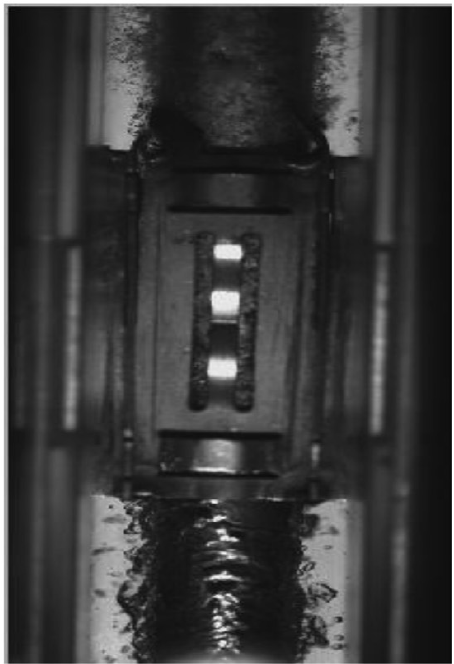
\includegraphics[width=0.25\linewidth]{img/intro/liu_CHF.png}
}
\caption{Visualization of a DNB-type boiling crisis on a rod with a mixing grid by Liu \etal \cite{liu_critical_2021}. The fluid is R134a at $P=2184~$kPa, $G = 2076~\debm$ , $T_{sat} - T_{L,in} = 22.8 \degC$. The insulating vapor blanket is clearly visible upstream the mixing grid.}
\label{fig:dnb_liu}
\end{figure}

\npar

According to Bricard (1995, \cite{bricard_modelisation_1995}), the LSD boiling crisis is well identified both by experimental and modeling approaches \cite{hewitt_phenomenological_1990} where the scientific community seems to have reached a consensus. On the contrary, DNB-type boiling crisis is much more debated since it results from local boiling phenomena including bubble dynamics at the wall and is still under thorough scientific investigation today \cite{kossolapov_experimental_2021, demarly_new_2020, richenderfer_experimental_2018, bloch_study_2016, bloch_phenomenological_2013}.


\subsection{Boiling Curves}

The boiling crisis phenomenon has been reported among the first times in the pioneering work of Nukiyama \cite{nukiyama_maximum_1966} who observed the variety of heat transfer regimes occurring during boiling and identified the maximum accessible heat flux as the Critical Heat Flux. He summarized his findings on a so-called "boiling curve" representing the evolution of the wall temperature (or superheat) against the applied heat flux $\phi_{w}$ (Figure \ref{fig:nukiyama_curve}).

\begin{figure}[!h]
\centering
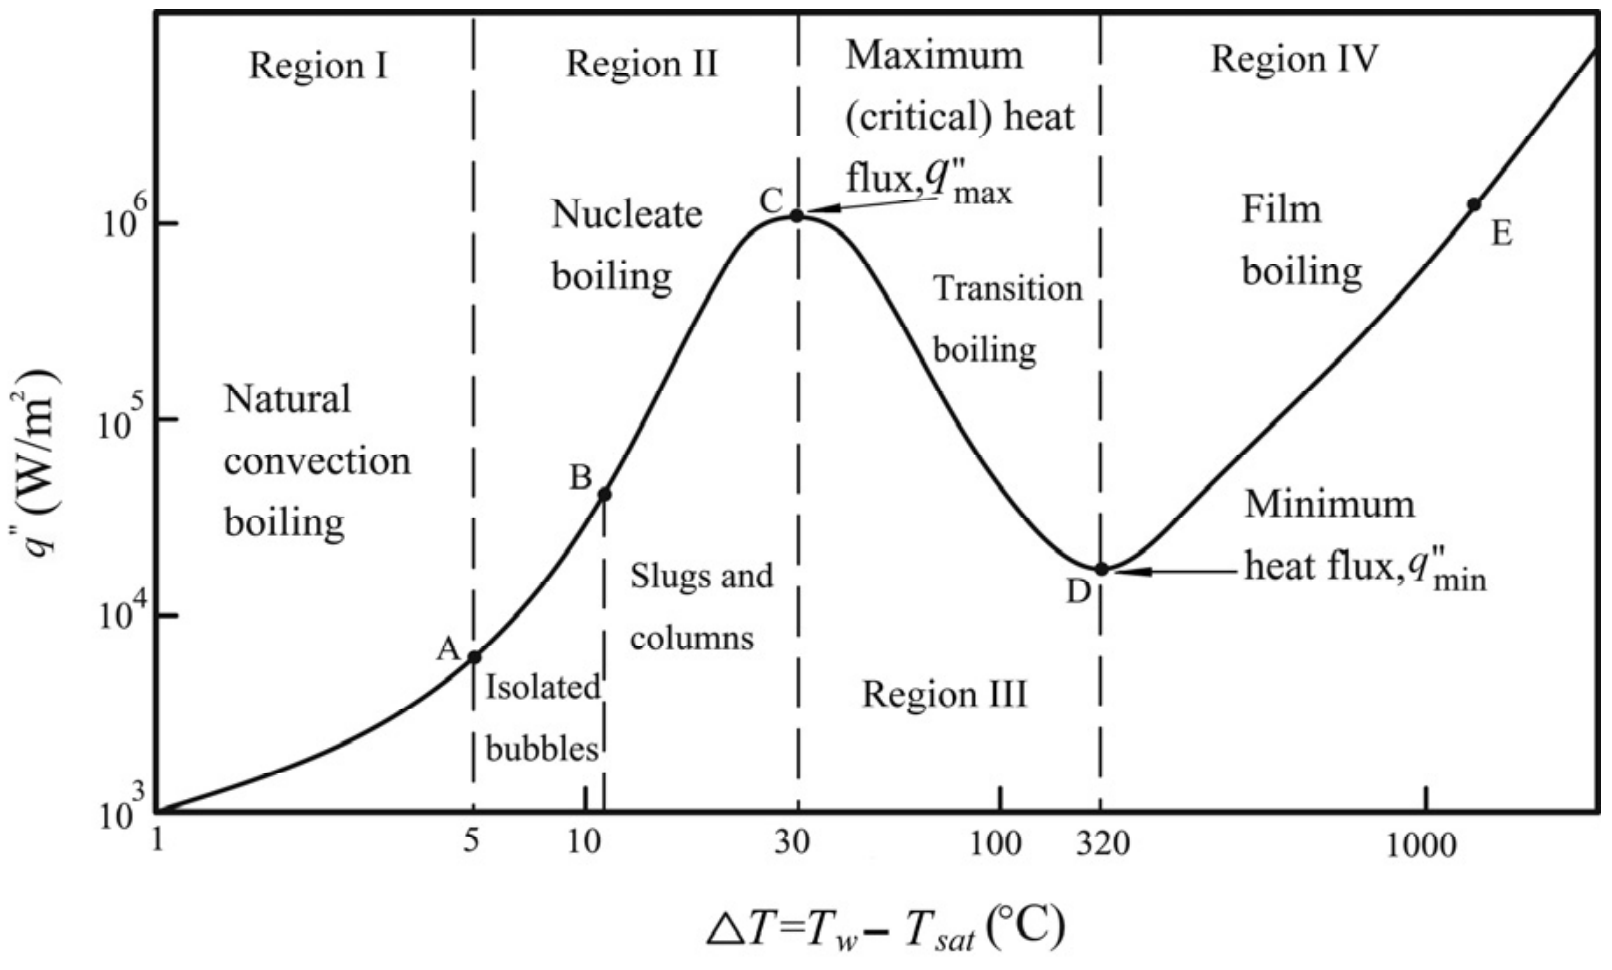
\includegraphics[width=0.7\linewidth]{img/intro/nukiyama.png}
\caption{Example of Nukiyama / boiling curve for water from \cite{faghri_10_2006}. Here $q''$ denotes the wall heat flux.}
\label{fig:nukiyama_curve}
\end{figure}


\npar

For a flux-controlled experiment, reaching the CHF triggers a nearly instantaneous transition from point C to point E (Figure \ref{fig:nukiyama_curve}) which graphically shows the violent increase in wall temperature that can damage the heater.


\section{Current Industrial Treatment of the Boiling Crisis}
\label{sec:intro_chf_indus}

Even if boiling can be a very efficient way of increasing the global heat transfer between a solid wall and surrounding liquid, the existence of the CHF as an upper limit over which the heater material integrity is threatened represents a huge physical limitation that has to be anticipated. Figure \ref{fig:chf_fuel} shows an example of fuel damage after undergoing a boiling crisis.


\begin{figure}[!h]
\subfloat[Post-BC damage on a rod]{
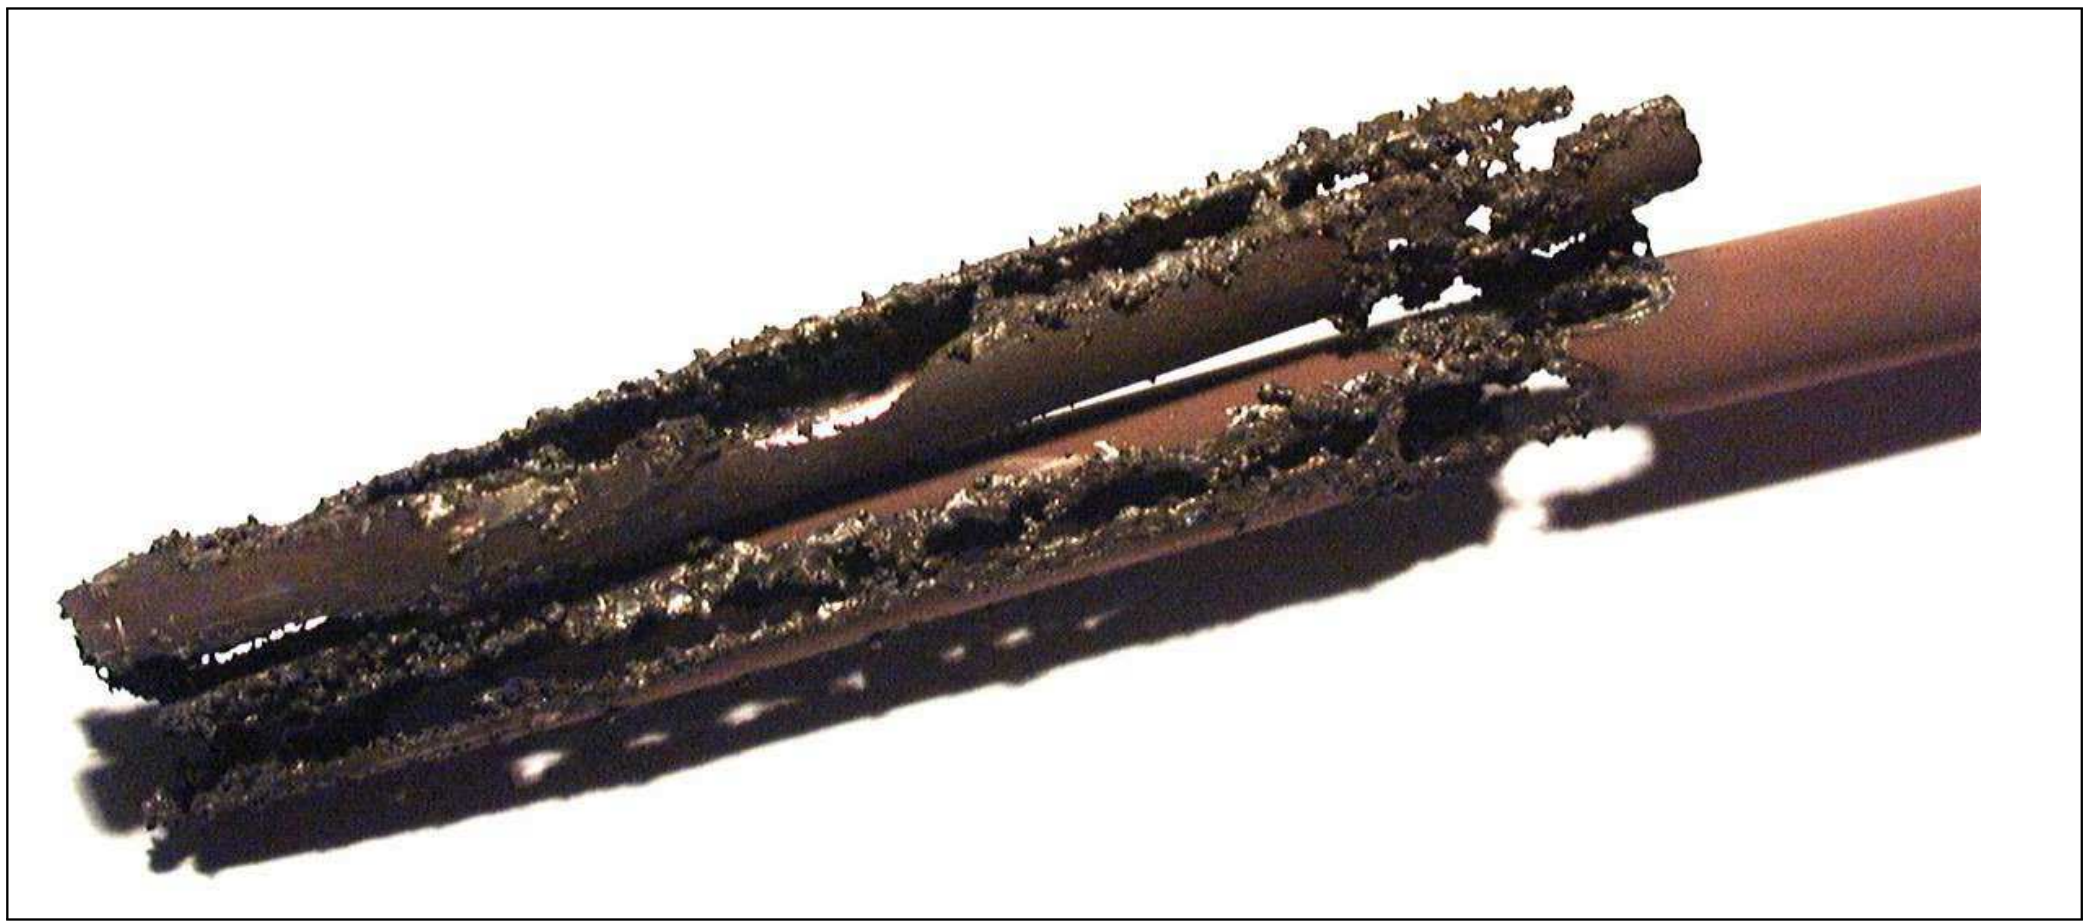
\includegraphics[width=0.5\linewidth]{img/intro/chf_rod.png}
}
\subfloat[Post-BC damage on an assembly (deformation not due to the BC)]{
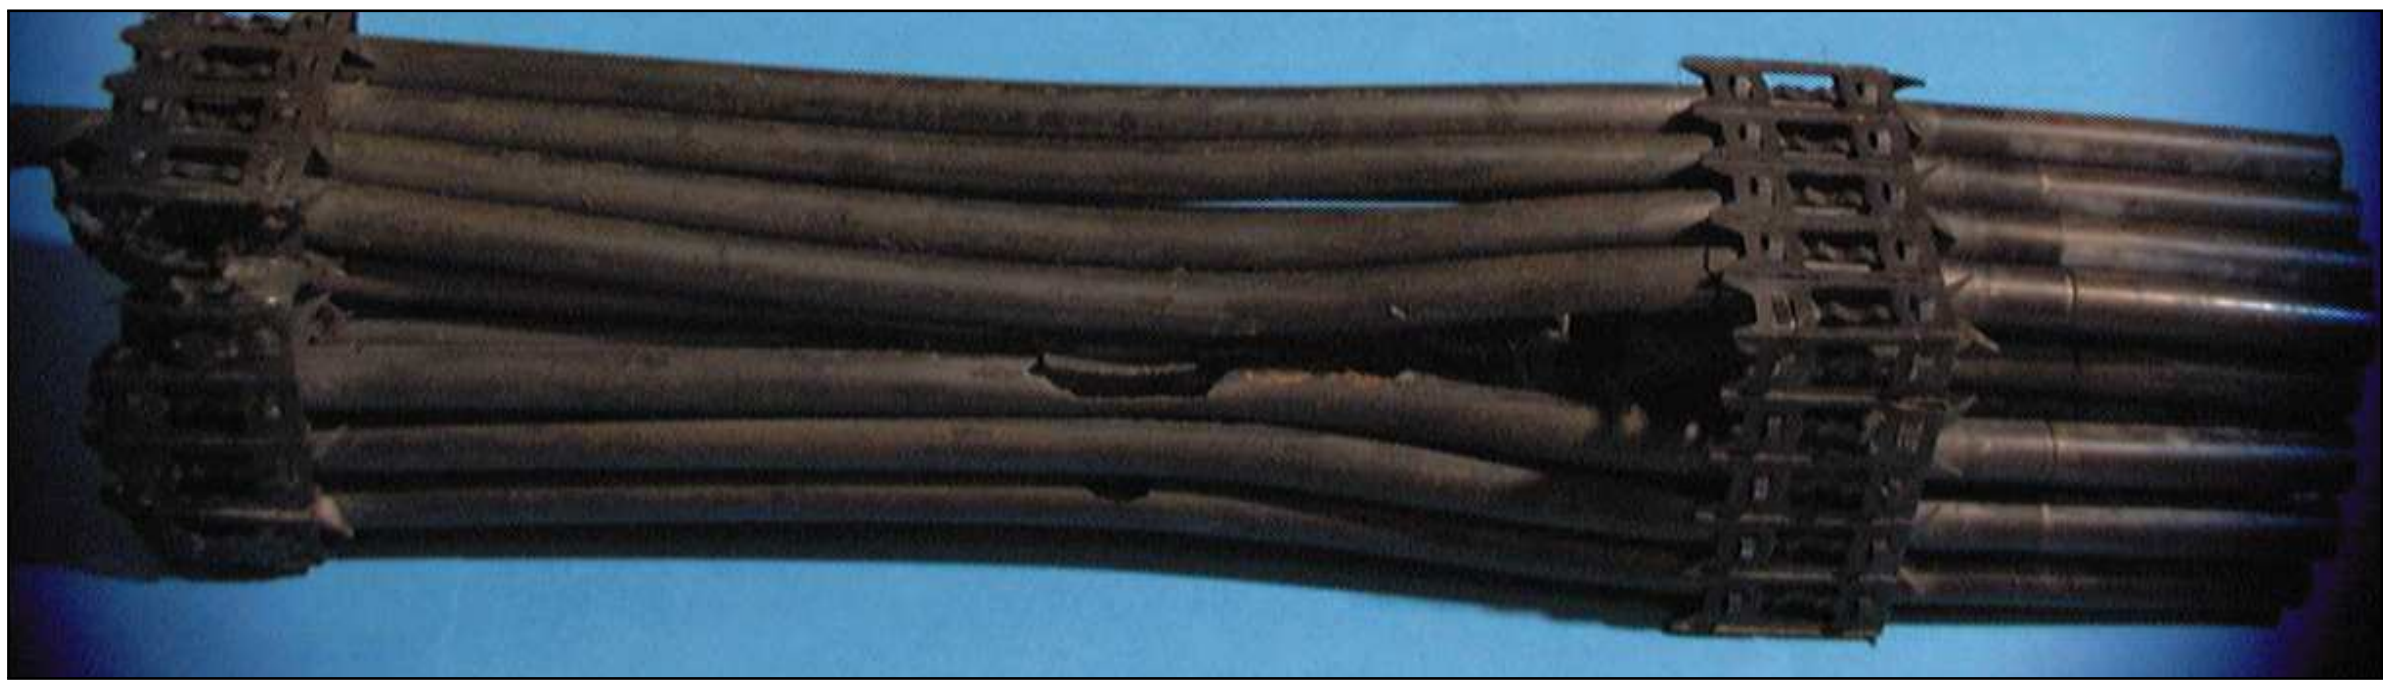
\includegraphics[width=0.5\linewidth]{img/intro/chf_assembly.png}
}
\caption{Damaged electrically heated components (used for CHF experimental tests in PWR conditions) after the boiling crisis (from CEA Omega experiment \cite{faccanoni_etude_2008}).}
\label{fig:chf_fuel}
\end{figure}

\npar

Any nuclear power unit operator, such as EDF, consequently has to prevent the occurrence of DNB in the core to ensure the full integrity of the nuclear fuel rods. Safety margins imposed by the french Nuclear Safety Authority (ASN) have to be respected at all time. Otherwise, the nuclear unit will have to be stopped in order to prevent any incident or accident. Such constraints represent a very challenging aspect for nuclear core thermal-hydraulics which primary goal is to be able to anticipate and predict the value of the CHF for a large range of operating conditions.

\npar

Earlier, we mentioned the fact that the DNB was still a very debated phenomenon over which a general scientific agreement has still to be reached. Therefore, CHF predictions for safety studies are currently achieved using dedicated experimental correlations. Using experiments on a nearly full-scale assembly ($5 \times 5$ electrically heated rods, grids, 4\ m height, water at 155\ bar, etc.), values of the CHF are measured in a large variety of operating conditions that covers the expected ranges for industrial operations. An empirical correlation based on those results is then constructed for the specific test geometry, usually of the form:

\begin{equation}
\phi_{w,CHF} = f\parth{P, G, L_{g}, D_{h}, x_{eq}}
\end{equation}
where $P$ is the pressure, $G$ the total mass flux, $L_{g}$ the distance between two grids (Figure \ref{fig:fuel_assembly}), $D_{h}$ the hydraulic diameter and $x_{eq}$ the thermodynamic quality.


\npar

This correlation is then used in multidimensional codes based on porous medium approaches (to avoid fine representation of the geometry), where the scale of a computation cell is usually that of a "sub-channel" (Figure \ref{fig:subchannel_sketch}) \ie the space between four rods.


\begin{figure}[!h]
\centering
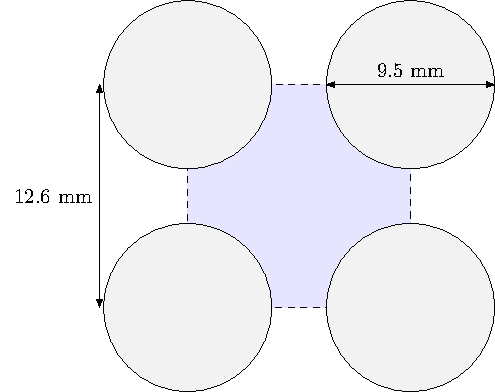
\includegraphics[width=0.4\linewidth]{img/intro/subchannel.pdf}
\caption{Sketch of a sub-channel in a rod bundle (dashed lines). The equivalent hydraulic diameter here is $D_{h}=11.78\ $mm.}
\label{fig:subchannel_sketch}
\end{figure}

\npar

Using the average thermal-hydraulics values of the flow at the scale of the subchannel, the dedicated correlation then estimates CHF in the cell which can be compared to the applied heat flux $\phi_{w}$ to estimate the \textbf{Departure to Nucleate Boiling Ratio} (DNBR) $\phi_{w} / \phi_{w,CHF}$ that gives the safety margin to the boiling crisis. For EDF, those numerical studies are conducted using the THYC code \cite{aubry_thyc_1995}.

\section{Towards Local Predictions of the CHF Using Computational Multi-Fluid Dynamics}

Investigating the boiling crisis physics has showed that the associated time-space scale was sometimes lower than 1\ ms and 1\ mm \cite{bloch_study_2016}, \ie smaller than the sub-channel scale. Achieving wall-boiling modeling at those scales is impossible with traditional safety studies codes and thus put the light onto Computational Multi-Fluid Dynamics (CMFD), which recent improvements over the past decades (model formulations, computational capacity, meshing techniques, etc.) has demonstrated its capability of simulating nearly industrial-scaled situations.

\npar

With CMFD codes, simulations of multiphase flows can be conducted at small local scales that are interesting to achieve:
\begin{itemize}
\item Finer descriptions of the multiphase flow structure and phase-change ;\
\item More detailed relationship between the wall local thermal-hydraulics properties and the boiling crisis using dedicated models including new physical phenomena related to wall boiling.
\end{itemize} 

At EDF R\&D, the in-house CFD code \textit{code\_saturne} has its own module dedicated to multiphase flows: NEPTUNE\_CFD \cite{guelfi_neptune_2007}. NEPTUNE\_CFD is the chosen numerical tool to investigate the modeling and simulation of the boiling crisis at CFD scale.


\section{Contents of This Thesis}

In this thesis, we want to address the problem of boiling crisis prediction using CFD in PWR conditions. This can be summed up in the following question:

\npar

\begin{center}
\textit{Is it nowadays possible to reach a proper modeling of the wall boiling phenomenon to predict boiling crisis occurrence in PWR using CFD simulations ?}
\end{center}
%
%\npar
%
%By simulating boiling flows in representative industrial conditions using NEPTUNE\_CFD, the validity of the present formulation of the code are assessed.
%
%\npar
%
%This leads us to further investigate the modeling of wall boiling in CFD codes using Heat Flux Partitioning (HFP) models and to propose a new formulation following a detailed study of the different physical parameters at stake. This is concluded by a discussion over the boiling crisis prediction using such models. 
%
%\npar
%
%Finally, geometries closer to the industrial configuration are studied to evaluate the difficulties involved by the specific design in PWR cores, notably regarding the presence of grids and mixing vanes (Figure \ref{fig:fuel_grid}).

\npar

This manuscript is organized as follows. \textbf{Part I} is dedicated to boiling flow simulations using NEPTUNE\_CFD:

\begin{itemize}
\item \textbf{Chapter \ref{chap:ncfd}} details the constitutive equations and the different closure laws used in the 7.0 version of NEPTUNE\_CFD. 

\item \textbf{Chapter \ref{chap:debora}} presents the DEBORA experimental database that will be used for CFD validation. Some analyses regarding the database consistency and physical implications are proposed.

\item \textbf{Chapter \ref{chap:debora_ncfd}} compares the simulation results obtained using NEPTUNE\_CFD with the DEBORA experiment. This allows to identify the strengths and weaknesses of the current modeling for boiling dispersed bubbly flows.

\end{itemize}


Following those investigations, \textbf{Part II} focuses on the development of a new Heat Flux Partitioning (HFP) model:

\begin{itemize}
\item \textbf{Chapter \ref{chap:HFP_bib}} briefly presents some bibliographic aspects regarding the modeling of wall boiling heat transfer.

\item \textbf{Chapter \ref{chap:bub_dyn}} then investigates in details the dynamics of bubble boiling at the wall. A particular care is given to the modeling of the bubble force balance to reach a representative description of the nucleated bubble movement.

\item \textbf{Chapter \ref{chap:HFP_Assembling}} discusses the different closure laws required to complete the Heat Flux Partitioning model and gathers experimental measurements for their assessment. The formulation of the new model is finally presented.

\item \textbf{Chapter \ref{ch:HFP_validation}} presents validation aspects of the model with comparisons to fine experimental measurements and wall temperature predictions from different literature databases.

\item \textbf{Chapter \ref{ch:to_CHF}} discusses perspectives regarding the prediction of the Critical Heat Flux using Heat Flux Partitioning models.
\end{itemize}

Finally, \textbf{Part III} investigates the impact of mixing vanes over the boiling flow:

\begin{itemize}
\item \textbf{Chapter \ref{chap:debora_agate_prom}} studies the DEBORA-Promoteur and AGATE-Promoteur experiments of a boiling and single-phase flow in a tube including mixing vanes. Analyses of the measurements are conducted to further understand the structure of boiling flows in PWR.

\item \textbf{Chapter \ref{chap:prom_ncfd}} presents NEPTUNE\_CFD simulations of the tube and mixing vanes case. Comparisons to the experiments evaluates the capacity of CFD to properly capture the effect of such geometries.
\end{itemize}

\textbf{Chapter \ref{ch:conclusion}} closes this manuscript by summarizing the different conclusions of the presented work and details the different perspectives emerging from the presented results.